\documentclass[10pt]{exam}

\usepackage{amssymb, amsmath, amsthm, mathrsfs, multicol, graphicx}
\usepackage{tikz}
\usetikzlibrary{calc}

\def\d{\displaystyle}
\def\?{\reflectbox{?}}
\def\b#1{\mathbf{#1}}
\def\f#1{\mathfrak #1}
\def\c#1{\mathcal #1}
\def\s#1{\mathscr #1}
\def\r#1{\mathrm{#1}}
\def\N{\mathbb N}
\def\Z{\mathbb Z}
\def\Q{\mathbb Q}
\def\R{\mathbb R}
\def\C{\mathbb C}
\def\F{\mathbb F}
\def\A{\mathbb A}
\def\X{\mathbb X}
\def\E{\mathbb E}
\def\O{\mathbb O}
\def\pow{\mathscr P}
\def\inv{^{-1}}
\def\nrml{\triangleleft}
\def\st{:}
\def\~{\widetilde}
\def\rem{\mathcal R}
\def\iff{\leftrightarrow}
\def\Iff{\Leftrightarrow}
\def\and{\wedge}
\def\And{\bigwedge}
\def\Vee{\bigvee}
\def\imp{\rightarrow}
\def\Imp{\Rightarrow}
\def\Fi{\Leftarrow}

\def\={\equiv}
\def\var{\mbox{var}}
\def\mod{\mbox{Mod}}
\def\Th{\mbox{Th}}
\def\sat{\mbox{Sat}}
\def\con{\mbox{Con}}
\def\bmodels{=\joinrel\mathrel|}
\def\iffmodels{\bmodels\models}
\def\dbland{\bigwedge \!\!\bigwedge}
\def\dom{\mbox{dom}}
\def\rng{\mbox{range}}
\DeclareMathOperator{\wgt}{wgt}

\def\circleA{(-.5,0) circle (1)}
\def\circleAlabel{(-1.5,.6) node[above]{$A$}}
\def\circleB{(.5,0) circle (1)}
\def\circleBlabel{(1.5,.6) node[above]{$B$}}
\def\circleC{(0,-1) circle (1)}
\def\circleClabel{(.5,-2) node[right]{$C$}}
\def\twosetbox{(-2,-1.5) rectangle (2,1.5)}
\def\threesetbox{(-2,-2.5) rectangle (2,1.5)}


\def\bar{\overline}

%\pointname{pts}
\pointsinmargin
\marginpointname{pts}
\marginbonuspointname{pts-bns}
\addpoints
\pagestyle{head}
% \printanswers

\firstpageheader{Math 228}{\bf Homework 11 - Extra Credit}{Due: Friday, November 30}

\def\vertexsize{4 pt}
\newcommand{\vtx}[2]{node[fill,circle,inner sep=0 pt, minimum size=\vertexsize,label=#1:#2]{}}
\newcommand{\va}[1]{\vtx{above}{#1}}
\newcommand{\vb}[1]{\vtx{below}{#1}}
\newcommand{\vr}[1]{\vtx{right}{#1}}
\newcommand{\vl}[1]{\vtx{left}{#1}}
\renewcommand{\v}{\vtx{above}{}}

\begin{document}
\noindent \textbf{Instructions}: This is an extra homework assignment for those of you looking to boost your homework grade. There are \numquestions\, exercises that total \numpoints\, points. You do not have to complete the entire assignment to get credit. However, these problems are also a nice review for the final. Same rules as usual -- turn in your work on separate sheets of paper.  You must justify all your answers for full credit.

As usual, you are encouraged to work with classmates on the assignment, but make sure your final write-up is in your own words.  You are not permitted to use the Internet to search for answers or use answers someone else has given you.
 
\begin{questions}

\question[2] Your little brother thinks he knows everything, even about graph theory.  He reminds you that the \emph{degree sequence} of a graph is a the list of degrees of the vertices in a graph, in non-increasing order (largest to smallest). He claims he has drawn a graph with degree sequence $(3,3,2,2,2,2,1)$.  Prove your little brother is wrong.
  \begin{solution}
    The sum of the degrees of his graph would be $15$.  But this would also be twice the number of edges, which needs to be a whole number.
  \end{solution}


\question[10] Your brother calls you back later to discuss his graph. ``Oh right,'' he says.  ``I meant $(3,3,2,2,2,2,2)$, and what's more\ldots'' and suddenly the call is dropped.  Assuming your brother really has drawn such a graph, which of the following are necessary, impossible, or possible (but not necessary)?  In each case, justify your answer.

\begin{parts}
  \part His graph is isomorphic to $G = (V,E)$ where $V = \{a,b,c,d,e,f,g\}$ and $E = \{ab, ac, ag, bc, cd, de, df, ef, fg\}$ (using the shorthand $xy$ for the edge $\{x,y\}$).
  \begin{solution}
    This is possible, as this graph does have that degree sequence, but it is not necessary, since there are other graphs not isomorphic to this that have the same degree sequence.
  \end{solution}
  \part His graph is connected.
  \begin{solution}
    This is possible but not necessary.  There is a non-connected graph with this degree sequence (a copy of $C_3$ together with a copy of $K_4$ with one edge removed).
  \end{solution}
  \part If his graph is connected, then it has an Euler path but not an Euler cycle.
  \begin{solution}
    This is necessary.  The graph has exactly two vertices with odd degree, so we know there will be an Euler path starting at one and ending at the other.
  \end{solution}
  \part If his graph is connected and planar, it has exactly 3 faces.
  \begin{solution}
    This is necessary.  If a graph is planar, it satisfies Euler's formula.  There are $7$ vertices, and there must be 9 edges, so we have $7 - 9 + f = 2$, which implies that $f = 3$.
  \end{solution}
  \part His graph has chromatic number 2.
  \begin{solution}
    I was almost certain this was impossible, until I tried to prove it, which led to the following example of a graph with that degree sequence and chromatic number 2: start with a 6-cycle, and then put the last vertex adjacent to two vertices distance two apart.   
  \end{solution}
\end{parts}


%Good:

\question[4] Can you distribute conjunctions over disjunctions?  Disjunctions over conjunctions?  Let's find out.  Remember, two statements are logically equivalent if they are true in exactly the same cases.
\begin{parts}
  \part Are the statements $P \vee (Q \and R)$ and $(P \vee Q) \and (P \vee R)$ logically equivalent?
  \begin{solution}
    Yes they are.  We prove this by showing that their truth tables are identical:
    \begin{center}
        \begin{tabular}{c|c|c||c||c}
    $P$ & $Q$ & $R$ & $P \vee (Q \and R)$ & $(P \vee Q) \and (P \vee R)$\\ \hline
    T & T & T & T & T\\
    T & T & F & T & T \\
    T & F & T & T & T \\
    T & F & F & T & T \\
    F & T & T & T & T \\
    F & T & F & F & F \\
    F & F & T & F & F \\
    F & F & F & F & F
  \end{tabular}
    \end{center}
  \end{solution}

  \part Are the statements $P \and (Q \vee R)$ and $(P \and Q) \vee (P \and R)$ logically equivalent?
  \begin{solution}
    It works again.  Here are the two truth tables which prove it:
        \begin{center}
        \begin{tabular}{c|c|c||c||c}
    $P$ & $Q$ & $R$ & $P \and (Q \vee R)$ & $(P \and Q) \vee (P \and R)$\\ \hline
    T & T & T & T & T\\
    T & T & F & T & T \\
    T & F & T & T & T \\
    T & F & F & F & F \\
    F & T & T & F & F \\
    F & T & F & F & F \\
    F & F & T & F & F \\
    F & F & F & F & F
  \end{tabular}
    \end{center}
  \end{solution}

\end{parts}


% %OK
% \question[4] While walking through a fictional forest, you stumble upon two trolls playing Stratego\textsuperscript{\textregistered}.  As you are well aware, all trolls are either knights who always tell the truth or knaves who always lie.  These two trolls tell you:
% \begin{itemize}
% \item[]Troll 1: If we are cousins, then we are both knaves.
% \item[]Troll 2: We are cousins or we are both knaves.
% \end{itemize}
%  Could both trolls be knights?  Prove your answer.  Your explanation should pay careful attention to the logical form of the statements, and perhaps even use truth tables.
% 
% \begin{solution}
% This is relatively easy to sort out if you use truth tables.  Let $P$ be ``We are cousins,'' and $Q$ be ``We are both knaves.''  We then get the truth table describing the statements:
% \centerline{
% \begin{tabular}{c|c|c|c}
% $P$ & $Q$ & $P \imp Q$ & $P \vee Q$ \\ \hline
% T & T & T & T\\
% T & F & F & T \\
% F & T & T & T \\
% F & F & T & F
% \end{tabular}
% }
% 
% Note that right away you can see that it is impossible for both trolls to be \emph{knaves}, since there is no case in which both of their statements are false.  From this we can conclude that the statement $Q$ is false!  So we are in rows 2 or 4.  But in each of these, one or the other troll is lying, so it is impossible for both to be knights.
% \end{solution}








\question[6] Suppose $G$ is a graph with 7 vertices.  Consider the statement:

\centerline{\textit{If $G$ has an Euler circuit, then there are at least 3 vertices with the same degree.}}

\begin{parts}
\part Write the \underline{first line} of a proof of the statement using each specified style of proof:

Direct proof:
\begin{solution}
Assume $G$ has an Euler circuit.
\end{solution}
Proof by contrapositive:
\begin{solution}
Assume there are at most 2 vertices with the same degree. (Assume it is not the case that at least 3 vertices have the same degree.)
\end{solution}
Proof by contradiction:
\begin{solution}
Assume $G$ has an Euler circuit but there are at most 2 vertices with the same degree.
\end{solution}
\part  Prove the statement using an appropriate style of proof.  Hint: what could the degrees be?
\begin{solution}
\begin{proof}
Proceed by contradiction.  Assume $G$ has an Euler circuit and that there are at most 2 vertices sharing the same degree.  Since $G$ has an Euler circuit, every vertex has \emph{even} degree.  Thus the possible degrees are 2, 4, and 6 (you cannot have larger degree since there are only 7 vertices).  Since there are at most 2 vertices sharing the same degree, there are at most 6 vertices.  This contradicts the assumption that $G$ has 7 vertices.
\end{proof}
\end{solution}
\end{parts}





\question[6] Tucker has started going to the gym to work out.  There are 15 different weight machines that he knows how to use.  Each day, he has enough time to do 8 exercises.  Obviously, Tucker would like to do a different workout routine each day.
\begin{parts}
  \part How many days can Tucker work out without repeating the same \emph{set} of 8 exercises, assuming all 8 exercises are different?  Explain.
  \begin{solution}
    There are $\binom{15}{8} = 6435$ different 8-elements subsets of the 15 machines.  Thus this is the number of days he could go before he had to repeat a set.
  \end{solution}
  \part How many days can Tucker work out without repeating the same \emph{sequence} of 8 exercises, assuming all 8 exercises are different? Explain how this is different from the previous part.
  \begin{solution}
    Here, the order in which Tucker does the exercises is enough to distinguish it from other sequences, even if the same set of exercises was done.  There are $P(15,8) = 259459200$ days before he would need to repeat a sequence.
  \end{solution}
  \part How would the answers to the previous questions change if Tucker allowed himself to do some of the exercises more than once (but still spend the same time; doing a total of 8 ``sets'')?  Find both numbers and say which corresponds to which part above.
  \begin{solution}
    If he was just interested in the (multi)set of exercises, not the order in which he did them, there would be $\binom{8+15-1}{15-1} = \binom{22}{14}$ choices (using 14 bars and 8 stars).  If the order in which he did the exercises matters, then there would be $15^8$ exercise routines.
  \end{solution}
\end{parts}



%OK, although the solution could be cleaned up.
\question[4] How many 10-digit numbers contain exactly four 1's, three 2's, two 3's and one 4?  Find the answer in two different ways to establish a binomial identity.
\begin{solution}

Some examples of acceptable outcomes: 1111222334, 1212121343, 4332221111, \ldots.  Each of these has 10 digits (as the questions states), and the number of each type of digit is the same.  It is just the arrangement that matters.  So does order matter here?  Maybe, but the order of what?  The digits?

How could I break the task of choosing an outcome into subtasks?  One way would be to first select what goes in the first digit, then in the second, etc.  In this sense order does matter.  Does that work?  Well there are 4 choices for the first digit.  For the second digit there are... well it depends on what I choose for the first digit.  So this doesn't work.  Let's try something else.

What if I first select where I put the 4.  It could go 1st, 2nd, etc.  There are 10 spots.  Thus 10, or maybe ${10 \choose 1}$.  Now where can I put the 3's.  It doesn't matter which 3 I place first, so here order does not matter.  I've already filled up one spot with a 4, so there are 9 spots left and I need 2 of them.  So ${9 \choose 2}$.  Ah, then ${7 \choose 3}$ to pick the three spots to put the 2's and ${4 \choose 4}$ choices of where to put the four 1's.  Now do I add or multiply?  Well to get my 10 digit number I need to do all these subtasks, not just one of them, so definitely multiply.  Thus the answer is
\[{10 \choose 1}{9 \choose 2}{7 \choose 3}{4 \choose 4} = 12600\]
Oh wait, what if I picked where the 1's went first?  There are ${10 \choose 4}$ spots, which leaves ${6 \choose 3}$ choices for where to put the 2's, and ${3 \choose 2}$ for the 3's and ${1 \choose 1}$ for the 4.  So now it looks like the answer should be
\[{10 \choose 4}{6 \choose 3}{3 \choose 2}{1 \choose 1}\]
Which is it?  Oh wait, those are the same.  Yay.

Let me check one more thing.  Did I get everything?  Did I double count?  Maybe let's try building one of the outcomes using the answer (the first one).  The first thing I do is pick on of 10 things.  10 spots.  So for example, I could pick this:
\[- - - - - ~ 4 - - - -\]
Next I pick 2 out of 9 things.  Those 9 things are\ldots, the 9 remaining spots.  What do I do with the 2 that I pick?  I put in 3's.  So maybe:
\[3 - - - - ~ 4 - 3 - -\]
Yeah, and I was right to use ${9 \choose 2}$ instead of $P(9,2)$ because it does not matter if I pick the 1st spot and then the 8th, or the 8th and then the 1st.  Next I choose 3 out of 7\ldots spots to\ldots put 2's into.  Maybe I get
\[3 - 2 2 - 4 - 3 - 2\]
and then put the 1's in the remaining 4 spots - ${4 \choose 4} = 1$, and yes, there is just one way to finish up:
\[3 1 22141312\]
And that is an acceptable outcome.  Double yay.
\end{solution}



\question[6] Consider the recurrence relation $a_n = 3a_{n-1} + 10a_{n-2}$.

\begin{parts}
  \part Find the general solution to the recurrence relation.  That is, find a closed formula for the $n$th term of the sequence, although this will have two parameters that would depend on initial conditions.
  \begin{solution}
    The recurrence relation has the characteristic polynomial $x^2 - 3x - 10$, which has roots $x = -2$ and $x = 5$.  Thus the general closed formula for this recurrence relation would be $a_n = a 5^n + b(-2)^n$, where $a$ and $b$ are constants that depend on the initial conditions.
  \end{solution}
  \part If this recurrence relation described the number of $1\times n$ paths you can make using squares and dominoes in various colors, how many colors of each would you have?
  \begin{solution}
    There would be 3 colors of squares and 10 colors of dominoes.  To make a $1\times n$ path, you could either start with one of 3 squares, followed by a path of length $n-1$ (of which there are $a_{n-1}$), or start with one of 10 dominoes followed by one of the $a_{n-2}$ many paths of length $n-2$.  So using the additive and multiplicative principles, this gives precisely the recurrence relation from this problem.
  \end{solution}
	\part Using the context from part (b), give initial conditions and find the specific closed formula for the recurrence relation subject to the initial conditions.
  \begin{solution}
    There will be 3 paths of length 1 (the three squares) and $3\cdot 3 + 10 = 19$ paths of length 2.  So the initial conditions are $a_1 = 3$ and $a_2 = 19$.  We could also work backwards and find that $a_0 = 1$, since that is how you could get $a_2 = 19$ using the recurrence relation.
    
    Now we solve the system of equations $1 = a+b$ and $3 = 5a-2b$ to get the closed formula $a_n = \frac{5}{7}(5)^n + \frac{2}{7}(-2)^n$.
  \end{solution}
\end{parts}



\question[4] Suppose that each day at noon, you eat 2 magic chocolate bunnies.  Over night, each bunny (not eaten) produces two more bunnies.  Let $B_n$ be the number of bunnies on day $n$ (at 8am, before you have eaten any).  Assume you started with 4 bunnies on day 1 at 8am (so $B_1 = 4$).  Prove, by induction, that $B_n < 3^{n}$ for all $n \ge 2$

\begin{solution}
  The sequence starts $4, 6, 12, 30, 84, \ldots$.  Here is the proof.
  
  \begin{proof}
    Let $P(n)$ be the statement ``$B_n < 3^{n+1}$''.  Note that $P(2)$ is true because $B_2 = 6$ which is less than $3^2 = 9$ (this is the base case).
    
    For the inductive case, assume $P(k)$ is true.  That is, assume $B_k < 3^k$.  Consider $B_{k+1} = 3(B_k - 2)$, since you get the number of bunnies on the next day by subtracting two then multiplying by 3.    Since $B_k < 3^k$, so is $B_k-2$.  But then $3(B_k-2)$ will be less than $3\cdot 3^k = 3^{k+1}$.
    
    Therefore, by the principle of mathematical induction, you will always have less than $3^n$ bunnies.  
  \end{proof}
\end{solution}

% 
% \question[6] Consider the binomial identity $\d {3 \choose 0} + {4 \choose 1} + {5 \choose 2} + \cdots + {3+n\choose n} = {4+n \choose n}$.  It might be helpful to ``find'' this in Pascal's Triangle.
% \begin{parts}
% 	\part Prove the identity using a combinatorial proof.  Hint: if you think about $n$-topping pizzas, which topping could be the ``last''?
% 	\part Prove the identity using mathematical induction.  Hint: you know a recurrence relation for the binomial coefficients---look at Pascal's Triangle.
% \end{parts}
% 
% 
% \begin{solution}
%   \begin{parts}
%     \part Consider the counting question: how many $n$-topping pizzas can you create if you have $n+4$ toppings?   One answer is clearly ${4+n \choose n}$.  Alternatively, you could break this up into cases by which topping is alphabetically the first one you don't choose.  If this is the 4th on your alphabetical list of toppings, then you picked 0 of the first three (and all the remaining $n$).  If this one is 5th on the list, then of the first 4, you must pick 1 (plus the remaining $n-1$).  If the last one is the 6th on the list, there are $n-2$ toppings you must choose, but of the first 5, you must choose 2.  And so on.  If you don't choose the last topping, then of the first $n+3$ you choose $n$.
%     \part Let $P(n)$ be the statement, $\d {3 \choose 0} + {4 \choose 1} + {5 \choose 2} + \cdots + {3+n\choose n} = {4+n \choose n}$.
% 
%     Base case: ${3 \choose 0} = 1 = {4 \choose 0}$ when $n = 0$.
% 
%     Inductive case.  Assume $P(k)$ is true.  Now
%     \[\d {3 \choose 0} + {4 \choose 1} + {5 \choose 2} + \cdots + {3+k\choose k} = {4+k \choose k}\]
%     so,
%     \[\d {3 \choose 0} + {4 \choose 1} + {5 \choose 2} + \cdots + {3+k\choose k} + {3+k+1 \choose k+1} = {4+k \choose k} + {3+k+1 \choose k+1}\]
%     but the left hand side is the same as $\d {4 + k+1 \choose k+1}$ by the recurrence relation ${n\choose k} = {n-1 \choose k-1} + {n-1 \choose k}$ (each entry in Pascal's triangle is the sum of the two entries above it).  Thus $P(k+1)$ is true.
% 
%     Therefore, by the Principle of Mathematical Induction, $P(n)$ is true for all $n \ge 0$
%   \end{parts}
% \end{solution}


% % What about the new Hamilton path exercise from the book?
% \question[6] We say that a graph has a {\em Hamilton path} if there is a path which visits each vertex exactly once (you do not need to use every edge in the path).
% \begin{parts}
%   \part Suppose a graph has a Hamilton path.  What is the maximum number of vertices of degree one the graph can have?  Explain why your answer is correct.
%
%   \begin{solution}
%     Note that a vertex of degree one can only be the start or the end of a Hamilton path - if we go {\em to} a vertex of degree one, we are stuck there - we cannot use the same edge to leave the vertex, because doing so would bring us back to a vertex we have already visited.  If a graph has a Hamilton path, it might start at a vertex of degree one, end at a vertex of degree one, but there cannot be any other vertices of degree one.  Therefore a graph with a Hamilton path can have at most two vertices of degree one.
%   \end{solution}
%
%   \part Find a graph which does not have a Hamilton path even though no vertex has degree one.  Explain why your example works.
%
%   \begin{solution}
%     There are many such graphs.  Here are two examples:
%
%     \begin{center}
%       \begin{tikzpicture}
%         \draw[thick] (-1,0) \v -- (0,1) \v -- (1, 0) \v -- (0, .33) \v -- (-1,0) -- (0,-.33) \v -- (1,0) -- (0,-1) \v -- (-1,0);
%       \end{tikzpicture}
%       \hspace{1in}
%       \begin{tikzpicture}
%         \draw[thick] (270:.5) \v -- (255:1) \v -- (285:1) \v -- (270:.5) -- (0,0) \v -- (135:.5) \v -- (150:1) \v -- (120:1) \v -- (135:.5) (0,0) -- (45:.5) \v -- (60:1) \v -- (30:1) \v -- (45:.5);
%       \end{tikzpicture}
%
%     \end{center}
%
%   \end{solution}
%
% \end{parts}







\question[4] In any graph, an \emph{independent set} is a subset of the vertices that are not adjacent to each other.  In other words, they are a set of vertices that could be colored the same in a proper vertex coloring.  Note that the empty set of vertices is independent.  How many different independent sets are there in $P_{10}$, the path of 10 vertices (9 edges)?  Hint: this is intended to be a question about sequences.  You should give a recursive definition for the number of independent sets in $P_n$ and explain why it is correct.

\begin{solution}
Start with $P_2$ (a pair of adjacent vertices).  There are exactly 3 independent sets: the empty set and the two sets that contain just one vertex.  Now for $P_3$, think of adding in 1 vertex to the end of $P_2$.  We could put this new vertex in the independent set or not.  If we keep it out, then each independent set we had before is still independent (so that is 3 already).  If we put it in, then we only have 2 choices: put the vertex on the other end in or not.  Thus there are a total of 5 independent sets.

Now the fun begins.  Add a 4th vertex on the end of the path to get $P_4$.  If we keep this vertex out, we could use any of the 5 independent sets of $P_3$.  If we put it in, then we cannot put the vertex next to it in, so we just need to get an independent set on the remaining two vertices.  But that looks just like $P_2$, and we know there are 3 independent sets.  So we have $8$ independent sets in $P_5$.

It's the Fibonacci recurrence.  The number of independent sets in $P_n$ is the number in $P_{n-1}$ (if we keep the new vertex out) plus the number in $P_{n-2}$ (if we put the new vertex in).  Following this up to $P_{10}$ we see there will be 144 independent sets.
\end{solution}



\question[4] Use your knowledge of sequences and graph theory to find the number of edges, vertices and triangular faces (all but the outside) of the $n$th figure in the sequence started below.  For example, the 1st figure has $e = 12$, $v = 7$, and $f = 6$.

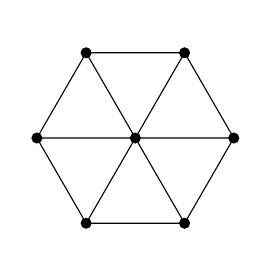
\begin{tikzpicture}[scale=1.25]
  \draw (0:0) \v;
  \foreach \x in {0,...,5}{
  \draw (0:0) -- (60*\x:1) \v -- (60*\x + 60: 1);
  }
\end{tikzpicture}
\hfill
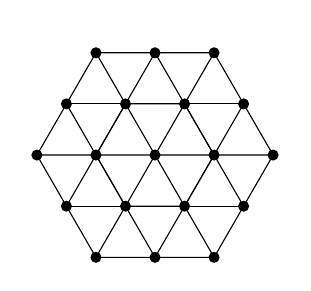
\begin{tikzpicture}[scale=.75]
  \draw (0:0) \v;
  \foreach \x in {0,...,5}{
  \draw (0:0) -- (60*\x:1) \v -- (60*\x + 60: 1) ;
  \draw (60*\x:1) -- (60*\x:2) \v -- (60*\x + 60:2);
  \draw ($ (60*\x:2)!.5!(60*\x + 60:2) $) \v -- ($ (60*\x+180:2)!.5!(60*\x + 120:2) $);
  }
\end{tikzpicture}
\hfill
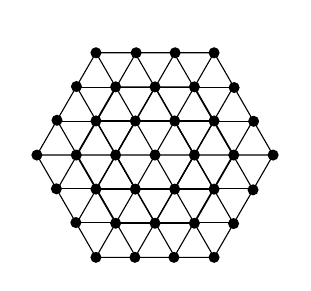
\begin{tikzpicture}[scale=.5]
  \draw (0:0) \v;
  \foreach \x in {0,...,5}{
  \draw (0:0) -- (60*\x:1) \v -- (60*\x + 60: 1) ;
  \draw (60*\x:1) -- (60*\x:2) \v -- (60*\x + 60:2);
  \draw ($ (60*\x:2)!.5!(60*\x + 60:2) $) \v -- ($ (60*\x+180:2)!.5!(60*\x + 120:2) $);
  \draw (60*\x:2) -- (60*\x:3) \v -- (60*\x + 60:3);
  \draw ($ (60*\x:3)!.33!(60*\x + 60:3) $) \v -- ($ (60*\x+180:3)!.33!(60*\x + 120:3) $);
    \draw ($ (60*\x:3)!.66!(60*\x + 60:3) $) \v -- ($ (60*\x+180:3)!.66!(60*\x + 120:3) $);
  }
\end{tikzpicture}
\hfill
$\cdots$

\begin{solution}
  First, we find the number of vertices in the $n$th figure to be $v_n = 3n^2 +3n + 1$ (you can use polynomial fitting, or notice that every time you add a larger multiple of 6 and use triangular numbers).

  Of these vertices, there will be 6 with degree 2 (the corners), $6n-6$ with degree 4 (the sides) and the rest, $3n^2 - 3n$ with degree 6.  Adding up the degrees and dividing by 2 gives the number of edges: $e_n = 9n^2 + 3n$.

  Finally, we can use Euler's formula to find the number of triangles.  However, since we don't want to count the outside, we would have
  \[f_n = 1 + 9n^2 + 3n - (3n^2 + 3n + 1) = 6n^2.\]
\end{solution}




\question[4] Use the \emph{deletion-contraction recurrence} and mathematical induction to prove that the chromatic polynomial of any tree with $n$ vertices is $k(k-1)^{n-1}$.  Hint: you should use the standard induction technique of considering a leaf and its edge.  

\begin{solution}
  Let $P(n)$ be the statement, ``All trees with $n$ vertices have chromatic polynomial $k(k-1)^{n-1}$''.  We will prove that $P9n)$ is true for all $n \ge 1$.
  
  Base case: A tree with one vertex is just a single vertex.  The chromatic polynomial for such a tree is $k$, which is $k(k-1)^(n-1) = k(k-1)^0$.
  
  Inductive case: Assume that $P(j)$ is true for some arbitrary $j \ge 1$ (we don't use $k$ since that is usually the variable in the chromatic polynomial).  That is, assume all trees with $j$ vertices have chromatic polynomial $k(k-1)^{j-1}$.  Now consider an arbitrary tree $G$ with $j+1$ vertices.  Let $v_0$ be a leaf of the tree, and $e$ the edge incident to $v_0$. Look at the graphs $G-e$ and $G/e$.  We know that $P(G,k) = P(G - e,k) - P(G/e,k)$.  The graph $G/e$ is a tree with $j$ vertices, so $P(G/e,k) = k(k-1)^{j-1}$.  
  The graph $G-e$ is a tree with $j$ vertices together with an isolated vertex $v$, so it's chromatic polynomial will be $P(G-e,k) = k(k-1)^{j-1}k$ (since $v$ can be colored with $k$ different colors for each coloring of the tree). 
  
  Putting this all  together gives
  \[
  P(G,k) = P(G-e,k) - P(G/e,k) = k^2(k-1)^{j-1} - k(k-1)^{j-1}. 
  \]
  We can factor out a $k(k-1)^{j-1}$ to get $k(k-1)^{j-1}(k-1)$ which gives us the desired $k(k-1)^j$.
  
  Therefore, by the principle of mathematical induction, $P(n)$ is true for all $n \ge 1$.
\end{solution}


\question[6] Consider the graph below.

\begin{center}
  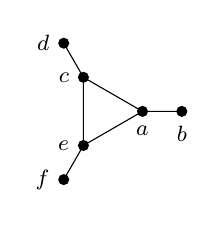
\begin{tikzpicture}[scale=.5]
    {\footnotesize
    \draw (0:1) \vb{$a$} -- (0:2) \vb{$b$} (0:1) -- (120:1) \vl{$c$} -- (120:2) \vl{$d$} (120:1) -- (240:1) \vl{$e$} -- (240:2) \vl{$f$} (240:1) -- (0:1);
    }
  \end{tikzpicture}
\end{center}
\begin{parts}
  \part Find the chromatic polynomial of the graph using only the multiplicative principle.  Explain why your answer is correct.
  \begin{solution}
    Start with vertex $a$.  There are $k$ choices for the color of $a$.  For each of these, there are $k-1$ choices for $c$, and then $k-2$ choices for $e$.  Each of $b$, $d$, and $f$ have $k-1$ choices (they just cannot be the same color as their single neighbor).  Thus the chromatic polynomial is $k(k-1)^4(k-2)$.
  \end{solution}
  \part Show how to use the \emph{deletion-contraction recurrence} to find the chromatic polynomial. Hint: there is an edge you can select that will allow you to use the result from the previous question.
  \begin{solution}
    Select the edge $ac$ (or either of the other two edges in the triangle).  If we delete this edge, we get a tree with $6$ vertices, so the chromatic polynomial is $k(k-1)^5$.  On the other hand, if we contract this edge, we get a tree with 5 vertices, so the chromatic number is $k(k-1)^4$.  The deletion-contraction recurrence says that the chromatic number of our original graph is then 
    \[
    k(k-1)^5 - k(k-1)^4
    \] 
    which agrees with our previous solution (factor out $k(k-1)^4$).
  \end{solution}
  \part Show how to use the Principle of Inclusion Exclusion to find the chromatic polynomial.  You might need to be careful, since not all edges behave the same way.
  \begin{solution}
    The idea here is that we start with $k^6$ colorings, then remove those that color the vertices of one or more edges the same.  
    
    First, consider how many colorings there are when any of the 6 edges are chosen and we color the two vertices of that edge identically.  There will be $k^5$ such colorings for each of these edges, so this group all together will have $\binom{6}{1}k^5 = 6k^5$ colorings.
    
    What if we pick two edges?  Now there are $k^4$ colorings for each pair of edges, so a total of $\binom{6}{2}k^4 = 15k^4$.
    
    If we pick 3 edges, we need to be careful.  If the three edges are those of the triangle, then there are $k^4$ colorings.  However, if any of the edges are not in the triangle, then there will be $k^3$ colorings.  All together then, this group has $k^4 + (\binom{6}{3}-1)k^3 = k^4 + 19k^3$ colorings.
    
    If we pick 4 edges, then if all three triangle edges are chosen, there would be $k^3$ colorings.  If not, then $k^2$ colorings.  So this group has $3k^3 + (\binom{6}{4}-3)k^2 = 3k^3+12k^2$.
    
    For 5 edges, there would be $k^2$ colorings if the three edges of the triangle were chose, but just $k$ if not.  So this give $3k^2 + (\binom{6}{5}-3)k = 3k^2 + 3k$.
    
    Finally, when all 6 edges are chosen, we have $k$ colorings.
    
    All together, we have:
    \[
    k^6 - \left[6k^5 - 15k^4 + (k^4 + 19k^3) - (3k^3 + 12k^2) + (3k^2 + 3k) - k\right]
    \]
    which we can simplify to 
    \[k^6 - 6k^5 + 14k^4 - 16k^3 + 9k^2 - 2k\]
    which is indeed what you get when you multiply out the polynomial from part (a).
  \end{solution}
\end{parts}


% \question[6] Whenever we have counted colorings of graphs (i.e., the chromatic polynomial) we have only considered \emph{labeled} graphs.  If the graph is not labeled, then which color belongs to which vertex is not important.  For example, coloring the path $P_4$ as red, yellow, red, blue (from left to right) is now the \emph{same} as coloring it blue, red, yellow, red.  However, this is a different coloring from red, blue, red, yellow.
% \begin{parts}
%   \part How many ways can you properly color an unlabeled $K_4$ using 7 colors?  How does this compare to the number of ways to color the labeled $K_4$?
%   \part How many ways can you properly color an unlabeled $P_4$ using 7 colors?
%   \part Explain why you cannot do the same thing you did for $P_4$ to count the number of 7-colorings of $P_3$.  Then count the number of colorings of (unlabeled) $P_3$ another way.
% \end{parts}




% % Could be left off:
% \question[4] An inventory list consists of 115 items, each on its own numbered line, each marked ``available'' or ``unavailable.'' There are 60 items marked available. Show that there are at least two available items in the list exactly four lines apart.
% \begin{solution}
% 	Assume for a contradiction that there are no items marked available exactly 4 items apart. To do this, let us consider two different sets. The first set will be the number of available items: \[a_1,a_2,...,a_60\] and the second set will be the number of items that cannot be marked as available \[a_1+4,a_2+4,...a_{60}+4\]. Now, each of these sets has exactly 60 items and must be separate items on the overall list. However, there are only 115 items on the list, which means that at least 2 items from each set must be the same item. Therefore, there must be at least two available items in the list exactly four items apart.
% \end{solution}







% \bonusquestion[4] {\bf BONUS:} Clu D. Tector was lecturing on methods for detecting counterfeit coins. To illustrate a point he removed four coins from his pocket, one of which is either heavier or lighter than the rest (in other words, it was counterfeit). He then pulled a fifth coin from his pocket and said it was a ``good'' coin. Next produced a balance scale and challenged the audience to suggest a plan for determining, in the fewest possible weighings, which of the four original coins was the counterfeit. He claimed you could do it in no more than two weighings. Describe how you would have to weigh the coins such that you would only have to only weigh the coins twice.
% \begin{solution}
% 	First, let's label each of the coins. The first four will be $A,B,C,D$ while the good coin will be $G$. Let's first measure $A,B$ against $C, G$. If the scale is balanced then we got lucky and $D$ is the counterfeit coin. Next, weigh $D$ against $G$ to figure out if it is heavy or light. However, it may be the case that that $A+B > C+G$ or $A+B < C+G$. If the first case is true then $D$ is a good coin, and either $C$ is light or $B$ or $A$ is heavy. Thus, a second weighting of $B$ against $A$ tells which coin is counterfeit. If $A=B$ then $C$ was the counterfeit and was lighter and if $A \not=B$ then whichever one weighed more is the counterfeit and is heavier. Similarly for $A+B<C+G$. In this case, either $C$ is heavy or $A$ or $B$ is light. Weigh $A$ against $B$ and if they are equivalent then $C$ is heavy. If not, then whichever one weighs less is the counterfeit and is lighter than the rest.
% \end{solution}
\end{questions}




\end{document}
